\documentclass[10pt]{article}
\usepackage[a4paper, margin=2cm]{geometry}
%\usepackage{fullpage}
\usepackage[T1]{fontenc}
\usepackage[utf8]{inputenc}
\usepackage{graphicx}
\usepackage{mathpazo}
\pagenumbering{arabic}
\usepackage{siunitx}
\usepackage{amsmath}
\usepackage{mathtools} % Para poder usar "\Aboxed"
\usepackage{cancel} % Para usar "\cancel", de https://tex.stackexchange.com/questions/537955/how-do-cross-out-text-in-math-mode
\usepackage{multicol}
\usepackage[spanish]{babel}
\usepackage{steinmetz}
\DeclareSIUnit\voltampere{VA}
\DeclareSIUnit\var{VAr}
\setlength\parindent{0pt} % no indent

% Numbering pages on the right footer:
% (https://tex.stackexchange.com/questions/153167/how-to-set-page-number-at-right-footer)
\usepackage{fancyhdr}
% Turn on the style
\pagestyle{fancy}
\fancyhf{} % sets both header and footer to nothing
\renewcommand{\headrulewidth}{0pt} % To remove the top horizontal line created by default by "fancyhdr", from here: https://tex.stackexchange.com/questions/13896/how-to-remove-the-top-horizontal-bar-in-fancyhdr
% Set the right side of the footer to be the page number
\fancyfoot[R]{\thepage}


\usepackage{minibox} % Para poder partir el texto en 2 líneas usando "underbrace" u "overbrace", info aquí: https://tex.stackexchange.com/questions/8680/how-can-i-insert-a-newline-in-a-framebox


\usepackage{xparse} % For "overbrace/underbrace but with an arrow instead", from https://tex.stackexchange.com/questions/8720/overbrace-underbrace-but-with-an-arrow-instead

% Para poner flechas sobre los signos de igual, de aquí: https://tex.stackexchange.com/questions/8720/overbrace-underbrace-but-with-an-arrow-instead
\NewDocumentCommand{\overarrow}{O{=} O{\uparrow} m}{%
  \overset{\makebox[0pt]{\begin{tabular}{@{}c@{}}#3\\[0pt]\ensuremath{#2}\end{tabular}}}{#1}
}
\NewDocumentCommand{\underarrow}{O{=} O{\downarrow} m}{%
  \underset{\makebox[0pt]{\begin{tabular}{@{}c@{}}\ensuremath{#2}\\[0pt]#3\end{tabular}}}{#1}
}





\begin{document}

\large{\textbf{Ejercicio 5 de la colección de problemas}}

\vspace{3mm}
\large{\textbf{Enunciado}}:

\vspace{3mm}
Analizar el circuito de la figura mediante el método de las mallas, obteniendo la corriente de cada una de las ramas. Con este resultado, calcular la diferencia de potencial entre A y B, y realizar un balance de potencias comparando la potencia de los elementos activos y la de los elementos pasivos.

\begin{minipage}{0.75\linewidth}
  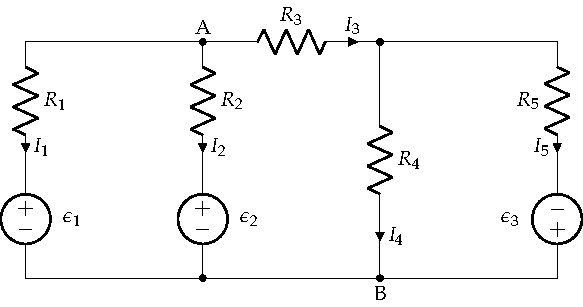
\includegraphics[scale=1.2]{figs/mallas2.pdf}
\end{minipage}
\begin{minipage}{0.25\linewidth}
    \textbf{Datos}:
    \vspace{2mm}
    
    $R_1 = R_2 = \qty{1}{\ohm}$\\ 
    $R_3 = \qty{2}{\ohm}$\\
    $R_4 = \qty{3}{\ohm}$\\
    $R_5=\qty{4}{\ohm}$\\
    $\epsilon_1=\qty{118}{\volt}$\\
    $\epsilon_2 = \qty{236}{\volt}$\\
    $\epsilon_3 = \qty{118}{\volt}$    
\end{minipage}

\vspace{4mm}

\hrulefill

\vspace{5mm}
\textbf{Solución}:
\vspace{4mm}

Se usan tres corrientes de malla con giro a derechas, de nombre (de
izquierda a derecha), $I_a$, $I_b$ e $I_c$. Escribiendo el sistema de
ecuaciones del método de las mallas en forma matricial:
\begin{equation*}
  \begin{bmatrix}
    2 & -1 & 0 \\
    -1 & 6 & -3 \\
    0 & -3 & 7
  \end{bmatrix}
  \cdot
  \begin{bmatrix}
    I_a\\
    I_b\\
    I_c
  \end{bmatrix}
  =
  \begin{bmatrix}
    -118\\
    236\\
    118
  \end{bmatrix}
\end{equation*}
cuya solución es:
\begin{align*}
  I_a &= \qty{-32}{\ampere}\\
  I_b &= \qty{54}{\ampere}\\
  I_c &= \qty{40}{\ampere}
\end{align*}

Estableciendo las relaciones entre las corrientes de rama y las
corrientes de malla, y sustituyendo, se llega a la conclusión de que:

\begin{align*}
  I_1 &= -I_a=\boxed{\qty{32}{\ampere}}\\
  I_2 &= I_a - I_b=-32-54=\boxed{\qty{-86}{\ampere}}\\
  I_3 &= I_b=\boxed{\qty{54}{\ampere}}\\
  I_4 &= I_b - I_c=54-40=\boxed{\qty{14}{\ampere}}\\
  I_5 &= I_c=\boxed{\qty{40}{\ampere}}
\end{align*}

\vspace{4mm}

\emph{Se recomienda comprobar que estos resultados cumplen la 1LK en
  los nudos del circuito, para asegurarse de que la resolución es
  correcta.}

\vspace{4mm}

La diferencia de potencial entre A y B es:
\begin{equation*}
  U_{AB} = I_3 \cdot R_3 + I_4 \cdot R_4 = 54\cdot 2+14\cdot 3= \boxed{\qty{150}{\volt}}
\end{equation*}

La potencia entregada por los generadores del circuito es:

\begin{align*}
  P_{\epsilon_1} &= \epsilon_1 \cdot (-I_1) = -\qty{3,776}{\kilo\watt}\\
  P_{\epsilon_2} &= \epsilon_2 \cdot (-I_2) = \qty{20,296}{\kilo\watt}\\
  P_{\epsilon_3} &= \epsilon_3 \cdot I_5 = \qty{4,72}{\kilo\watt}\\
  P_\epsilon &= P_{\epsilon_1} + P_{\epsilon_2} + P_{\epsilon_3} = \boxed{\qty{21,24}{\kilo\watt}}  
\end{align*}

Es importante recordar que el criterio de signos de un generador considera que la potencia entregada es positiva cuando la corriente sale del generador por su terminal positivo. Por tanto, $I_1$ e $I_2$ son empleadas con un signo negativo. En consecuencia, la potencia del generador $\epsilon_1$ es negativa, lo que quiere decir que este generador funciona como receptor (absorbe potencia). Ahora bien, dado que $I_2$ tiene valor negativo (es decir, circula en sentido contrario al indicado en la figura), la potencia del generador $\epsilon_2$ es positiva, de forma que este generador actúa como tal.

\vspace{3mm}

La potencia disipada por las resistencias es:

\begin{align*}
  P_{R_1} &= I_1^2 \cdot R_1 = \qty{1,024}{\kilo\watt}\\
  P_{R_2} &= I_2^2 \cdot R_2 = \qty{7,396}{\kilo\watt}\\
  P_{R_3} &= I_3^2 \cdot R_3 = \qty{5,832}{\kilo\watt}\\
  P_{R_4} &= I_4^2 \cdot R_4 = \qty{588}{\watt}\\
  P_{R_5} &= I_5^2 \cdot R_5 = \qty{6,4}{\kilo\watt}\\
  P_R &= \sum_i P_{Ri} = \boxed{\qty{21,24}{\kilo\watt}}  
\end{align*}

Comprobamos que se cumple el balance de potencias.


\end{document}
